\chapter{Skalar- und Kreuzprodukt}

% ... (Skalarprodukt Section bleibt gleich) ...
\section{Skalarprodukt}

Das Skalarprodukt zweier Vektoren \(\vec{a}\) und \(\vec{b}\) wird in dieser Veranstaltung als \(\left\langle \vec{a}, \vec{b} \right\rangle\) notiert. Andere gebräuchliche Schreibweisen sind \(\vec{a} \circ \vec{b}\) oder \(\vec{a} \cdot \vec{b}\). Eine Grundvoraussetzung für die Berechnung des Skalarprodukts ist, dass die beiden Vektoren dieselbe Anzahl von Komponenten besitzen, also aus demselben Vektorraum \(\mathbb{R}^n\) stammen.

Das Skalarprodukt wird berechnet, indem die korrespondierenden Komponenten der beiden Vektoren multipliziert und die resultierenden Produkte summiert werden. Für zwei Vektoren
\[ \vec{v} = \begin{pmatrix} v_1 \\ v_2 \\ \vdots \\ v_n \end{pmatrix} \quad \text{und} \quad \vec{w} = \begin{pmatrix} w_1 \\ w_2 \\ \vdots \\ w_n \end{pmatrix} \]
ist das Skalarprodukt definiert als:
\[ \left\langle \vec{v}, \vec{w} \right\rangle = v_1 \cdot w_1 + v_2 \cdot w_2 + \cdots + v_n \cdot w_n = \sum_{i=1}^{n} v_i \cdot w_i \]

\section{Kreuzprodukt}

Das Kreuzprodukt (auch Vektorprodukt genannt) ist eine mathematische Operation, die zwei Vektoren im dreidimensionalen Raum (\(\mathbb{R}^3\)) nimmt und einen neuen Vektor erzeugt. Dieser resultierende Vektor \(\vec{c} = \vec{a} \times \vec{b}\) steht senkrecht (orthogonal) auf der Ebene, die von den beiden ursprünglichen Vektoren \(\vec{a}\) und \(\vec{b}\) aufgespannt wird. Die Richtung des Ergebnisvektors wird durch die Rechte-Hand-Regel bestimmt.

Der Betrag (die Länge) des resultierenden Vektors \(||\vec{a} \times \vec{b}||\) entspricht der Fläche des Parallelogramms, das von den Vektoren \(\vec{a}\) und \(\vec{b}\) aufgespannt wird.

Für zwei Vektoren \(\vec{a} = \begin{pmatrix} a_1 \\ a_2 \\ a_3 \end{pmatrix}\) und \(\vec{b} = \begin{pmatrix} b_1 \\ b_2 \\ b_3 \end{pmatrix}\) im \(\mathbb{R}^3\) berechnet sich das Kreuzprodukt \(\vec{a} \times \vec{b}\) wie folgt:
\[ \vec{a} \times \vec{b} = \begin{pmatrix} a_1 \\ a_2 \\ a_3 \end{pmatrix} \times \begin{pmatrix} b_1 \\ b_2 \\ b_3 \end{pmatrix} = \begin{pmatrix} a_2 b_3 - a_3 b_2 \\ a_3 b_1 - a_1 b_3 \\ a_1 b_2 - a_2 b_1 \end{pmatrix} \]

\subsection{Berechnungsschema}
Das Schema zur Berechnung der Komponenten \(c_1, c_2, c_3\) des Kreuzprodukts \(\vec{c} = \vec{a} \times \vec{b}\) kann visualisiert werden. Die folgende Grafik zeigt eine Methode, die auf der Regel von Sarrus basiert.

\begin{figure}[h!] % Um die TikZ-Zeichnung in eine figure-Umgebung zu setzen
\centering % Zentriert die Zeichnung
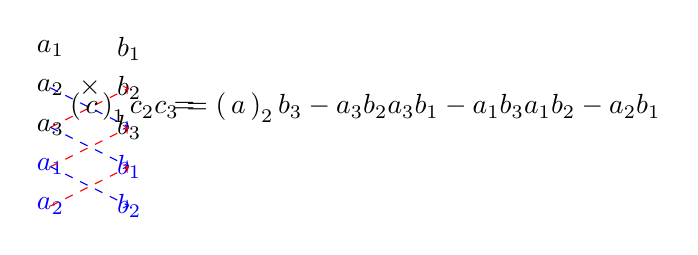
\begin{tikzpicture}

    \node at (0, 0) {\(a_1\)};
    \node at (0, -0.5) {\(a_2\)};
    \node at (0, -1) {\(a_3\)};
    \node at (0.5, -0.5) {\(\times\)};
    \node at (1, 0) {\(b_1\)};
    \node at (1, -0.5) {\(b_2\)};
    \node at (1, -1) {\(b_3\)};

    \node[text=blue] at (0, -1.5) {\(a_1\)};
    \node[text=blue] at (0, -2) {\(a_2\)};

    \node[text=blue] at (1, -1.5) {\(b_1\)};
    \node[text=blue] at (1, -2) {\(b_2\)};

    % Pfeile für c_1
    \draw[dashed, blue, ->] (0,-0.5) -- (1, -1);   % a_2 * b_3
    \draw[dashed, red, ->] (0,-1) -- (1, -0.5);   % a_3 * b_2

    % Pfeile für c_2
    \draw[dashed, blue, ->] (0,-1) -- (1, -1.5);  % a_3 * b_1 (rep.)
    \draw[dashed, red, ->] (0,-1.5) -- (1, -1);  % a_1 (rep.) * b_3

    % Pfeile für c_3
    \draw[dashed, blue, ->] (0,-1.5) -- (1, -2); % a_1 (rep.) * b_2 (rep.)
    \draw[dashed, red, ->] (0,-2) -- (1, -1.5); % a_2 (rep.) * b_1 (rep.)

    \node at (1.7, -0.75) {\(=\)};
    \node at (4, -0.75) {\(\begin{pmatrix}
        c_1 \\ c_2 \\ c_3
    \end{pmatrix} = \begin{pmatrix}
        a_2b_3 - a_3b_2 \\
        a_3b_1 - a_1b_3 \\
        a_1b_2 - a_2b_1
    \end{pmatrix}\)}; % Ergebnisvektor etwas verschoben für bessere Lesbarkeit

\end{tikzpicture}
\caption{Berechnungsschema des Kreuzprodukts nach der Regel von Sarrus. Die ersten beiden Komponenten jedes Vektors werden unterhalb wiederholt (hier in blau dargestellt).}
\label{fig:kreuzprodukt_sarrus_user}
\end{figure}

\subsubsection*{Erläuterung der Zeichnung zur Kreuzproduktberechnung}

Die oben dargestellte Grafik (siehe Abbildung \ref{fig:kreuzprodukt_sarrus_user}) veranschaulicht eine Methode zur Berechnung des Kreuzprodukts \(\vec{c} = \vec{a} \times \vec{b}\), die oft als Erweiterung der Regel von Sarrus bezeichnet wird. So wird die Zeichnung verwendet:

\begin{enumerate}
    \item \textbf{Komponenten aufschreiben:} Die Komponenten der beiden Vektoren \(\vec{a} = \begin{pmatrix} a_1 \\ a_2 \\ a_3 \end{pmatrix}\) und \(\vec{b} = \begin{pmatrix} b_1 \\ b_2 \\ b_3 \end{pmatrix}\) werden nebeneinander notiert.
    \item \textbf{Komponenten wiederholen:} Die ersten beiden Komponenten jedes Vektors (\(a_1, a_2\) und \(b_1, b_2\)) werden unterhalb der ursprünglichen drei Komponenten erneut aufgeschrieben. In der Zeichnung sind diese wiederholten Komponenten zur Verdeutlichung blau markiert.
    \item \textbf{Produkte bilden und Komponenten berechnen:} Nun werden die Komponenten des Ergebnisvektors \(\vec{c} = \begin{pmatrix} c_1 \\ c_2 \\ c_3 \end{pmatrix}\) durch diagonale Multiplikation bestimmt:
    \begin{itemize}
        \item \textbf{Für \(c_1\):}
        Man betrachtet die zweite und dritte Zeile der ursprünglichen Komponenten.
        Die blau gestrichelte Linie von \(a_2\) nach \(b_3\) zeigt das Produkt \(+a_2 b_3\).
        Die rot gestrichelte Linie von \(a_3\) nach \(b_2\) zeigt das Produkt \(-a_3 b_2\).
        Somit ist \(c_1 = a_2 b_3 - a_3 b_2\).

        \item \textbf{Für \(c_2\):}
        Man betrachtet die dritte Zeile der ursprünglichen Komponenten (\(a_3, b_3\)) und die erste Zeile der wiederholten Komponenten (\(a_1, b_1\), in blau).
        Die blau gestrichelte Linie von \(a_3\) (Original) nach \(b_1\) (blau, wiederholt) zeigt das Produkt \(+a_3 b_1\).
        Die rot gestrichelte Linie von \(a_1\) (blau, wiederholt) nach \(b_3\) (Original) zeigt das Produkt \(-a_1 b_3\).
        Somit ist \(c_2 = a_3 b_1 - a_1 b_3\).

        \item \textbf{Für \(c_3\):}
        Man betrachtet die erste und zweite Zeile der wiederholten Komponenten (alle blau).
        Die blau gestrichelte Linie von \(a_1\) (blau, wiederholt) nach \(b_2\) (blau, wiederholt) zeigt das Produkt \(+a_1 b_2\).
        Die rot gestrichelte Linie von \(a_2\) (blau, wiederholt) nach \(b_1\) (blau, wiederholt) zeigt das Produkt \(-a_2 b_1\).
        Somit ist \(c_3 = a_1 b_2 - a_2 b_1\).
    \end{itemize}
    \item \textbf{Ergebnisvektor:} Die berechneten Werte \(c_1, c_2, c_3\) bilden die Komponenten des Kreuzproduktvektors, wie auf der rechten Seite der Zeichnung dargestellt.
\end{enumerate}
